\documentclass[12pt]{amsbook}
\usepackage{geometry}                % See geometry.pdf to learn the layout options. There are lots.
%\geometry{letterpaper}                   % ... or a4paper or a5paper or ... 
\geometry{a4paper, top=25mm, right=25mm, bottom=25mm}
%\geometry{landscape}                % Activate for rotated page geometry
\usepackage[parfill]{parskip}    % Activate to begin paragraphs with an empty line rather than an indent
\usepackage{relsize}             % Allows us to define \bigast
\usepackage{graphicx}
\usepackage{amssymb}
\usepackage{epstopdf}
%\usepackage{pause}
\usepackage{wasysym}            % Provides \checkmark
\usepackage[firstpage]{draft watermark}             % Allows the watermark stuff
\usepackage{wrapfig}
\DeclareGraphicsRule{.tif}{png}{.png}{`convert #1 `dirname #1`/`basename #1 .tif`.png}

\newcommand{\DD}{\displaystyle}

\begin{document}
\pagenumbering{gobble}       % This kills the page numbering

\SetWatermarkText{
\begin{minipage}[c][8cm]{8cm}
\begin{center}
 
\end{center}
\end{minipage}
}
\SetWatermarkScale{1.5}
\SetWatermarkColor[gray]{0.75}



\begin{center}
   \textsc{\large MATH 255, Exam 2}\\
\end{center}
\vspace{1cm}

\textbf{Name} \; \underline{\hspace{5cm}}

\vspace{1cm}

\textbf{Instructions} \; No notes, textbook, homework, or calculators may be used for this exam. The exam is designed to take 50 minutes and must be submitted at the end of the class period. All of your solutions should be easily identifiable and supporting work must be shown. You may use any part of this packet as scratch paper, but please clearly label what work you want to be considered for grading. Ambiguous or illegible answers will not be counted as correct.

\vspace{1cm}

\textbf{Problem 1} \; \underline{\hspace{.75cm}}/20

\vspace{.25cm}

\textbf{Problem 2} \; \underline{\hspace{.75cm}}/20

\vspace{.25cm}

\textbf{Problem 3} \; \underline{\hspace{.75cm}}/20

\vspace{.25cm}

\textbf{Problem 4} \; \underline{\hspace{.75cm}}/20

\vspace{.25cm}

\textbf{Problem 5} \; \underline{\hspace{.75cm}}/20

\vspace{.25cm}

\textbf{Bonus} \;\hspace{.9cm} \underline{\hspace{.75cm}}/10

\vspace{.25cm}

\textbf{Total} \;\hspace{1.1cm} \underline{\hspace{.75cm}}/100










\newpage

\textbf{Problem 1}

\vspace{.25cm}

\textbf{(i)} Is the following statement True or False? Justify your answer.
\begin{center}
If $f(x,y)$ is a scalar field with defined partial derivatives of all orders, 

then $\nabla f(x_0,y_0) = \textbf{0}$ (the zero vector) for all stationary points $(x_0,y_0)$.
\end{center}

\vspace{5cm}

\textbf{(ii)} Let $f(x,y) = x^3+y^3-3xy + 4$. Find all of the stationary points for $f$ and classify each as a local minimum, local maximum, or saddle point.








\newpage

\textbf{Problem 2}

\vspace{.25cm}

\textbf{(i)} Is the following statement True or False? Justify your answer.
\begin{center}
Let $A,B,C$ be $n\times n$ invertible matrices, and let $\sim$ denote similarity. Then:

if $A\sim B$, and $B\sim C$, then $\text{det}(A) = \text{det}(B)\text{det}(C)$.
\end{center}

\vspace{5cm}


\textbf{(ii)} Suppose $A$ is a $2\times 2$ matrix with eigenvalues $\lambda_1 = 3$ and $\lambda_2 = 2$, and with corresponding eigenvectors $\textbf{x}_1 = \left[\begin{array}{c} -1 \\ 1\end{array}\right]$ and $\textbf{x}_2 = \left[\begin{array}{c} -2 \\ 3 \end{array}\right]$. Find $A^2$.









\newpage

\textbf{Problem 3}

\vspace{.25cm}

\textbf{(i)} Let $z_1 = -\frac{\sqrt{2}}{2} + i\frac{\sqrt{2}}{2}$ and $z_2 = \frac{\sqrt{3}}{2}+i\frac{1}{2}$. Compute the following:
\begin{itemize}
\item[(a)] $z_1^{51}$ in Cartesian form.
\item[(b)] $z_1 z_2$ in polar form.
\item[(c)] $z_2^{-1}$ in Cartesian form.
\end{itemize}


\vspace{7cm}

\textbf{(ii)} Compute $\DD \int_C \left[y \; dx + \frac{\ln(y)}{x} \; dy\right]$ on the curve $y=e^{2x}$ from $x=0$ to $2$.




\newpage

\textbf{Problem 4}

\vspace{.25cm}

\textbf{(i)} Consider the vector field $\textbf{F}(x,y) = |x|\textbf{i} - |y|\textbf{j}$. Draw an approximation for this vector field in $\mathbb{R}^2$.


\vspace{8cm}

\textbf{(ii)} Find the minimum and and maximum of $f(x,y) = 2x-4y$ subject to the constraint $g(x,y) = x^2+y^2 = 5$. Clearly identify which point is the minimum and which is the maximum.









\newpage

\textbf{Problem 5}

\vspace{.25cm}

\begin{wrapfigure}{r}{0.3\textwidth} 
    \centering
    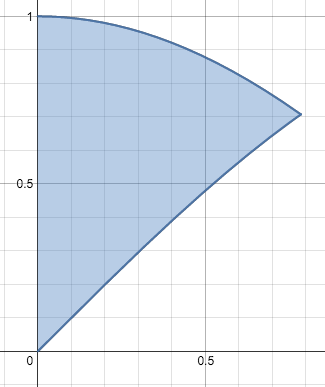
\includegraphics[scale=.5]{region.png}
\end{wrapfigure}

Let $R$ be the region in $\mathbb{R}^2$ shown to the right. It is bounded above by $y=\cos(x)$ and bounded below by $y=\sin(x)$.



(a) Find the area of $R$. 

\vspace{8cm}




(b) Suppose $R$ represents a lake in which frogs are known to reproduce. Let $\DD p(x,y) = \frac{5130}{((x-0.5)(y-0.3))^2+1}$ be the population density of tadpoles measured in tadpoles per meters squared in the lake. Set up \textit{\textbf{but do not evaluate}} the integral which gives the total number of tadpoles in the lake.














\newpage

\textbf{Bonus} 

Let $\textbf{F}$ be the same as in Problem 4(i). Find $\nabla\cdot \textbf{F}$ and $\nabla \times \textbf{F}$ at the following points.
\begin{itemize}
\item[(a)] $(1,1)$
\item[(b)] $(1,-1)$
\item[(c)] $(-1,1)$
\item[(d)] $(-1,-1)$.
\end{itemize}













\end{document}  